\documentclass[12pt, a4 paper]{article}
\usepackage{geometry}
\geometry{left=2cm, right=2cm, top=1.5cm, bottom=1.5cm}
\usepackage{amsmath}
\usepackage{amssymb}
\usepackage{amsfonts}
\usepackage{framed}
\usepackage{caption}
\usepackage{indentfirst}
\usepackage{graphicx}
\usepackage[colorlinks,linkcolor=blue]{hyperref}
\usepackage{pythonhighlight}
\usepackage[linesnumbered,boxed,ruled,commentsnumbered]{algorithm2e}%%算法包,注意设置所需可选项

\begin{document}

    %%%%%%%%%%%%%%%%%%%%%%%%%%%%%%%%%%%%%%   Q1   %%%%%%%%%%%%%%%%%%%%%%%%%%%%%%%%%%%%%%%%%
    \begin{framed}
        \section{[Q1]}
        Since last assignment, we talked about proximal gradient
        descent. Then we talk about geometric view of contrained 
        problems. After that, we talked about Lagrange problem and
        the Lagrange dual problem and how to relate the optimal
        $x^{\star}$ with $\lambda^{\star}$, $\upsilon^{\star}$. Besides,
        we dig deeper into KKT conditions and talked about strong duality.
        If $d^{\star}  = p^{\star}$, strong duality holds. From there,
        we talked about indicator function and convex conjugate which are 
        used to solve dual problem. Note that Fenchel duality is a more
        general way of Lagrangian duality.
    \end{framed}

    %%%%%%%%%%%%%%%%%%%%%%%%%%%%%%%%%%%%%%   Q2   %%%%%%%%%%%%%%%%%%%%%%%%%%%%%%%%%%%%%%%%%
    \begin{framed}
        \section{[Q2]}
        done
    \end{framed}

    %%%%%%%%%%%%%%%%%%%%%%%%%%%%%%%%%%%%%%   Q3   %%%%%%%%%%%%%%%%%%%%%%%%%%%%%%%%%%%%%%%%%
    \begin{framed}
        \section{[Q3]}
        \subsection{(a)}
        $$
        \partial \lVert x \rVert_{\infty} = u
        $$
        \indent Define $n$ as the index of the first maximum
        $\lvert x_{i} \rvert, \forall i$,
        if $\lvert x_{n} \rvert \geq \lvert x_{i} \rvert,
        \forall i $, we can have,
        $$
        u_{n} = \text{sign}(x)
        $$
        \indent else, $u_{n}=0$.\\
        \indent where $$\text{sign}(x) = \left\{
        \begin{aligned}
            &1, \text{ if } x \geq 0\\
            &-1, \text{else}
        \end{aligned}
        \right.
        $$

        \subsection{(b)}
        From $u^{T}x = \lVert x \rVert_{\infty}$, we can conclude,
        \begin{equation}
            \langle y-x, u \rangle = u^{T}y - u^{T}x = u^{T}y - \lVert x \rVert_{\infty}
        \end{equation}
        \indent Since $\lVert u \rVert_{1}=1$, we have $\lvert u_{1} \rvert + \lvert 
        u_{2} \rvert + \cdots + \lvert u_{n} \rvert = 1$.\\
        \indent Assume $\forall i, |y_{j}| \geq |y_{i}|$
        \begin{equation}
            u^{T}y = \sum\limits_{i}^{n} u_{i}y_{i} \leq \sum\limits_{i}^{n} |u_{i}|
            |y_{i}| \leq \sum\limits_{i}^{n} |u_{i}||y_{j}| \leq |y_{j}| \sum\limits
            ^{n}|u_{i}| = |y_{j}| = \lVert y \rVert_{\infty}
        \end{equation}
        \indent Hence, we can arrive at,
        \begin{align}
            \langle y-x, u \rangle &\leq \lVert y \rVert_{\infty} - 
            \lVert x \rVert_{\infty}\\
            f(x) + \langle y-x, u \rangle &\leq \lVert y \rVert_{\infty}\\
            f(x) + \langle y-x, u \rangle &\leq f(y)
        \end{align}
        \indent Therefore, $u$ must be subgradient.
        
        \subsection{(c)}
        If $u$ is a subgradient of $\lVert x \rVert_{\infty}$, then 
        it satisfy,
        \begin{align}
            \lVert y \rVert_{\infty} &\geq \lVert x \rVert_{\infty} +
            u^{T}y - u^{T}x\\
            \lVert y \rVert_{\infty} - u^{T}y &\geq \lVert x \rVert_{\infty}
            - u^{T}x
        \end{align}
        \indent Let $y=0$, we can have,
        \begin{align}
            0 \geq \lVert x \rVert_{\infty} - u^{T}x
        \end{align}
        \indent Let $y=2x$, we can have,
        \begin{align}
            \lVert x \rVert_{\infty} - u^{T}x \geq 0
        \end{align}
        \indent Hence, we can arrive at,
        \begin{equation}
            \lVert x \rVert_{\infty} = u^{T}x
        \end{equation}

        \indent Besides, we can dig further as follows,
        \begin{align}
            \lVert x \rVert_{\infty} &= u^{T}x \\
            &= \sum\limits_{i=1}^{n} u_{i}x_{i}\\
            &\leq \sum\limits_{i=1}^{n} \lvert u_{i} \rvert \lvert x_{i} \rvert\\
            &\leq \lVert x \rVert_{\infty} \lVert u \rVert_{1}
        \end{align}
        \indent Hence we can arrive at,
        \begin{equation}
            \lVert u \rVert_{1} \geq 1
        \end{equation}

        \indent Now, take $\lVert x \rVert_{\infty} = u^{T}x$ back to (6) we can
        get,
        \begin{align}
            \lVert y \rVert_{\infty} \geq u^{T}y
        \end{align}
        \indent Again, use the same trick as above, we can get,
        \begin{align}
            u^{T}y &\leq \lVert y \rVert_{\infty} \lVert u \rVert_{1}\\
            &\leq \lVert y \rVert_{\infty}
        \end{align}
        \indent we can get,
        \begin{equation}
            \lVert u \rVert_{1} \leq 1
        \end{equation}
        \indent Combine (15) with (19), we can get,
        \begin{equation}
            \lVert u \rVert_{1} = 1
        \end{equation}
        \indent Note (10) and (20) are exact two conditions
        needed to prove.
    \end{framed}

    %%%%%%%%%%%%%%%%%%%%%%%%%%%%%%%%%%%%%%   Q4   %%%%%%%%%%%%%%%%%%%%%%%%%%%%%%%%%%%%%%%%%
    \begin{framed}
        \section{[Q4]}
        \subsection{(a)}
        \begin{align}
            h_{B_{2}} (\upsilon) &= \sup\limits_{x \in B_{2}} \langle  x, \upsilon \rangle
        \end{align}
        \indent According to Cauchy-Schwartz inequality, we have,
        \begin{align}
            \langle  x, \upsilon \rangle &\leq \lVert x \rVert_{2} \cdot 
            \lVert \upsilon \rVert_{2} \\
            &\leq \lVert \upsilon \rVert_{2}
        \end{align}
        \indent where inequality (23) holds because in set $B_{2}$, $\lVert x 
        \rVert_{2} \leq 1$\\
        \indent Hence,
        $$
        h_{B_{2}} (\upsilon) = \lVert \upsilon \rVert_{2}
        $$

        \subsection{(b)}
        \begin{align}
            \lVert \upsilon \rVert_{2\star} &= 
            \sup\limits_{\lVert x \rVert_{2} \leq 1}  \langle x, \upsilon \rangle\\
            &\leq \sup\limits_{\lVert x \rVert_{2} \leq 1} \lVert x \rVert_{2}
            \lVert \upsilon \rVert_{2} \\
            &= \lVert \upsilon \rVert_{2}
        \end{align}
        \indent where, inequality (25) comes from Cauchy-Schwartz inequality. And $l_{2}$
        norm is a self-dual norm.

        \subsection{(c)}
        Let's assume $\forall i, \lvert \upsilon_{j} \rvert \geq \lvert \upsilon_{i} \rvert $
        \begin{align}
            h_{B_{1}}(\upsilon) &= \sup\limits_{x \in B_{1}} \langle x, \upsilon \rangle\\
            &=\sup\limits_{x \in B_{1}} \sum\limits_{i}^{n} \upsilon_{i}x_{i}\\
            &\leq \sup\limits_{x \in B_{1}} \sum\limits_{i}^{n} \lvert \upsilon_{i} \rvert
            \lvert x_{i} \rvert\\
            &\leq \lvert \upsilon_{j} \rvert \sup\limits_{x \in B_{1}} \sum_{i}^{n}
             \lvert x_{i} \rvert\\
            & = \lVert \upsilon \rVert_{\infty} 
        \end{align}
        \indent where inequality (30) is because $\lVert x \rVert_{1} \leq 1$.

        \subsection{(d)}
        Let's assume $\forall i, \lvert \upsilon_{j} \rvert \geq \lvert \upsilon_{i} \rvert $
        \begin{align}
            \lVert \upsilon \rVert_{1\star} &= \sup\limits_{ \lVert x \rVert_{1}\leq 1 }
            \langle x, \upsilon \rangle\\
            &= \sup\limits_{ \lVert x \rVert_{1}\leq 1 } \sum_{i}^{n} \upsilon_{i}x_{i}\\
            &= \sup\limits_{ \lVert x \rVert_{1}\leq 1 } \sum_{i}^{n} \lvert \upsilon_{i}
             \rvert \lvert x_{i} \rvert\\
            &= \lvert \upsilon_{j} \rvert \sup\limits_{ \lVert x \rVert_{1}\leq 1 }
            \sum_{i}^{n} \lvert x_{i} \rvert\\
            &= \lVert \upsilon \rVert_{\infty}
        \end{align}

        \subsection{(e)}
        \begin{align}
            h_{B_{\infty}}(\upsilon) &= \sup\limits_{\lVert x \rVert_{\infty \leq 1} }
            \langle x, \upsilon \rangle\\
            &= \sup\limits_{\lVert x \rVert_{\infty} \leq 1} \sum_{i}^{n} \upsilon_{i}x_{i}\\
            &= \sup\limits_{\lVert x \rVert_{\infty} \leq 1} \sum_{i}^{n} \lvert \upsilon
             \rvert \lvert x_{i} \rvert\\
            &= \lVert x \rVert_{\infty} \sup\limits_{\lVert x \rVert_{\infty} \leq 1}
            \sum_{i}^{n} \lvert \upsilon_{i} \rvert\\
            &= \sup\limits_{\lVert x \rVert_{\infty} \leq 1} \sum_{i}^{n} \lvert \upsilon_{i}
             \rvert\\
            &= \lVert \upsilon \rVert_{1}
        \end{align}

        \subsection{(f)}
        \begin{align}
            \lVert \upsilon \rVert_{\infty \star} &= \sup\limits_{\lVert x \rVert_{\infty \leq 1} }
            \langle x, \upsilon \rangle\\
            &= \sup\limits_{\lVert x \rVert_{\infty} \leq 1} \sum_{i}^{n} \upsilon_{i}x_{i}\\
            &= \sup\limits_{\lVert x \rVert_{\infty} \leq 1} \sum_{i}^{n} \lvert \upsilon
             \rvert \lvert x_{i} \rvert\\
            &= \lVert x \rVert_{\infty} \sup\limits_{\lVert x \rVert_{\infty} \leq 1}
            \sum_{i}^{n} \lvert \upsilon_{i} \rvert\\
            &= \sup\limits_{\lVert x \rVert_{\infty} \leq 1} \sum_{i}^{n} \lvert \upsilon_{i}
             \rvert\\
            &= \lVert \upsilon \rVert_{1}
        \end{align}

    \end{framed}

    %%%%%%%%%%%%%%%%%%%%%%%%%%%%%%%%%%%%%%   Q5   %%%%%%%%%%%%%%%%%%%%%%%%%%%%%%%%%%%%%%%%%
    \begin{framed}
        \section{[Q5]}
        \subsection{(a)}
        Since $\upsilon \in \partial f(x)$, we have,
        \begin{align}
            f(y) &\geq f(x) + \langle y-x,v \rangle\\
            \langle y,v \rangle - f(y) &\leq \langle x,v \rangle - f(x)
        \end{align}
        \indent Take $\sup$ for $y$ at both sides, we can get,
        \begin{align}
            \sup\limits_{y} \langle y,v \rangle - f(y) &\leq 
            \sup\limits_{y} \langle x,v \rangle - f(x)\\
            f^{\star}(v) &\leq \langle x,v \rangle -f(x)\\
            f^{\star}(v) + f(x) &\leq \langle x,v \rangle
        \end{align}
        \indent From Fenchel inequality, we can get,
        \begin{align}
            f^{\star}(v) + f(x) \geq \langle x,v \rangle
        \end{align}
        \indent Combined with (53) we can get,
        \begin{align}
            f^{\star}(v) + f(x) = \langle x,v \rangle
        \end{align}

        \indent Also, from Fenchel inequality, we can get
        \begin{align}
            f^{\star}(y) + f(x) &\geq \langle x,y \rangle\\
            f^{\star}(y) &\geq \langle x,v \rangle - f(x) + 
            \langle y-v, x \rangle\\
            f^{\star}(y) &\geq f^{\star}(v) + \langle y-v, x\rangle
        \end{align}
        \indent where, (58) holds because I take (55) into (57).


        \subsection{(b)}
        Let $g(x)=f^{\star}(x)$, since $x \in \partial g(v)$, according
        to conclusion from (a), we can have,
        \begin{align}
            v \in \partial g^{\star}(x)
        \end{align}
        \indent since we know $g^{\star} = f^{\star \star} = f$, we arrive
        at,
        \begin{align}
            v \in \partial f(x)
        \end{align}

    \end{framed}


    %%%%%%%%%%%%%%%%%%%%%%%%%%%%%%%%%%%%%%   Q6   %%%%%%%%%%%%%%%%%%%%%%%%%%%%%%%%%%%%%%%%%
    \begin{framed}
        \section{[Q6]}
        \subsection{(a)}
        Let's assume $d_{1}, d_{2} \in \text{set } D(x_{0})$, we have,
        \begin{align}
            d_{1}: f(x_{0} + t_{1}d_{1}) &\leq f(x_{0}), \quad \text{for some } t_{1} \\
            d_{2}: f(x_{0} + t+{2}d_{2}) &\leq f(x_{0}), \quad \text{for some } t_{2}
        \end{align}
        \indent Let's denote $x_{1}=x_{0}+t_{1}d_{1}$ and $x_{0}+t_{2}d_{2}=x_{2}$,
        by definition of convexity,
        \begin{align}
            f(\theta x_{1}+(1-\theta)x_{2}) \leq \theta f(x_{1}) + (1-\theta)f(x_{2})
            , \theta \in \left[ 0,1 \right]
        \end{align}
        \indent Therefore,
        \begin{align}
            f(x_{0}+\theta t_{1}d_{1} + (1-\theta)t_{2}d_{2}) &\leq f(x_{1}) +
            (1-\theta) f(x_{2})\\
            &\leq \theta f(x_{0}) + (1-\theta) f(x_{0})\\
            &= f(x_{0})
        \end{align}
        \indent Although $\theta \in \left[0,1\right]$, $\theta t_{1}$ and 
        $(1-\theta)t_{2}$ can be arbitrary number. Hence,
        \begin{align}
            \theta t_{1}d_{1} + (1-\theta)t_{2}d_{2} \in \mathbf{D},
            \quad \theta t_{1}, (1-\theta)t_{2} \in \mathbf{R}
        \end{align}
        \indent which indicates $\mathbf{D}$ is a convex cone.

        \subsection{(b)}
        Since $\lVert x \rVert_{2}^{2}$ is differentiable everywhere,
        \begin{align}
            \mathbf{D}(\boldsymbol{x}_{0}) &= \left\{ 
                \mathbf{d}: \langle \mathbf{d}, \nabla f(x_{0}) \rangle < 0
            \right\}\\
            &=\left\{ 
                \mathbf{d}: \langle \mathbf{d}, 2x_{0} \rangle < 0
                \right\}
        \end{align}

        \subsection{(c)}
        From $\lVert x_{0}+td \rvert_{1} \leq \lVert x_{0} 
        \rVert_{1}$, we can get,
        \begin{equation}
            \mathbf{d} = \left\{
                \begin{aligned}
                &-\text{sign}(x_{n}), &\text{ if } n \in \Gamma  \\
                &0, &\text{ if } n \notin \Gamma \\
                \end{aligned}
                \right.
        \end{equation}
        \indent where $\Gamma = \left\{n: x_{n} \neq 0 \right\}$.

        

    \end{framed}

    %%%%%%%%%%%%%%%%%%%%%%%%%%%%%%%%%%%%%%   Q7   %%%%%%%%%%%%%%%%%%%%%%%%%%%%%%%%%%%%%%%%%
    \begin{framed}
        \section{[Q7]}
        \subsection{(a)}
        According to KKT condtion (K1), we have,
        \begin{equation}
            (x-2)(x-4) \leq 0
        \end{equation}
        \indent the feasible set is $ \left\{x: 2 \leq x \leq 4 \right\} $

        \subsection{(b)}
        The Lagrangian for this problem is,
        $$
            L(x, \lambda) = x^{2}+1 + \lambda (x-2)(x-4)
        $$
        \indent According to KKT conditions (K4), we have,
        $$
        \frac{\partial{L}}{\partial x} = 2x + 2\lambda x - 6\lambda
        $$
        \indent Set it to 0, we can get $x$ as follows,
        $$
        x = \frac{3\lambda}{\lambda + 1}
        $$
        \indent Lagrange dual program is
        $$
        \mathop{\text{maximize}}_{\lambda} \frac{-\lambda^{3} +
        8\lambda^{2} + 10\lambda + 1}{(\lambda+1)^{2}}, \quad
        \text{subject to } \lambda \geq 0
        $$
        \indent Apprently, this will be maximize when $\lambda=2$,
        which, when substituted into the dual problem yields,
        $$
        d(\lambda^{\star}) = 5
        $$
        \indent Hence, the optimal $x^{\star}$ is \textbf{2}, accordingly,
        the value of the objective function at the minimizer is \textbf{5}.

        \subsection{(c)}
        {\centering
        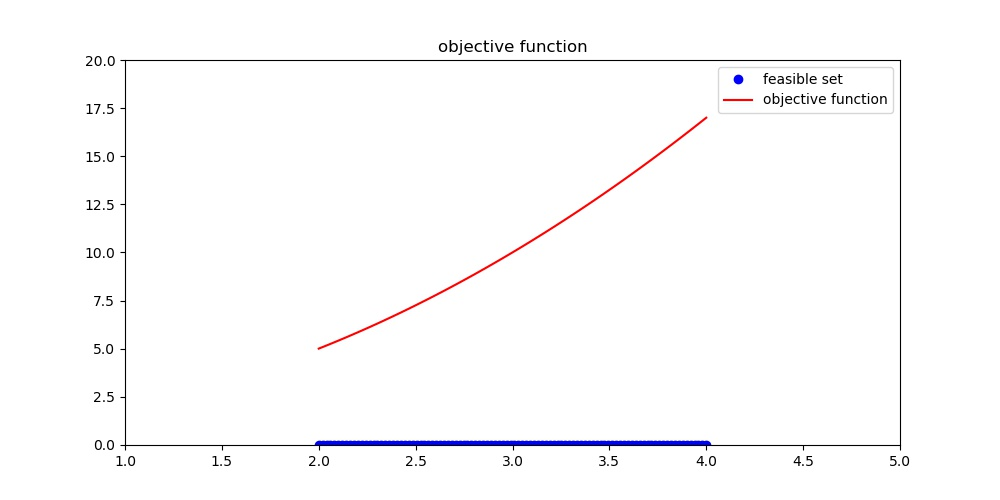
\includegraphics[width=10cm, height=5cm]{7c.jpg}
        \captionof{figure}{Plot of Objective Function} 
        }
        {\centering
        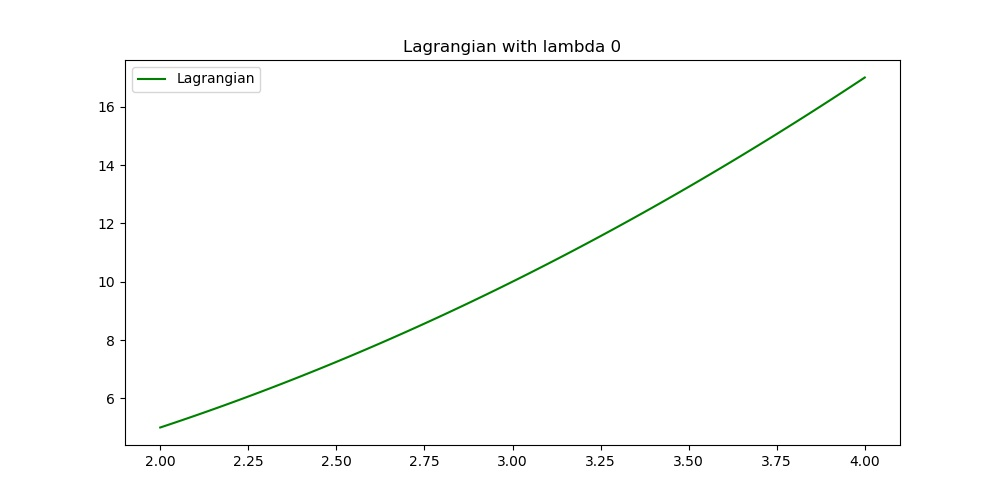
\includegraphics[width=10cm, height=5cm]{7c-lam0.jpg}
        \captionof{figure}{Plot of Lagrangian with $\lambda=0$} 
        }
        {\centering
        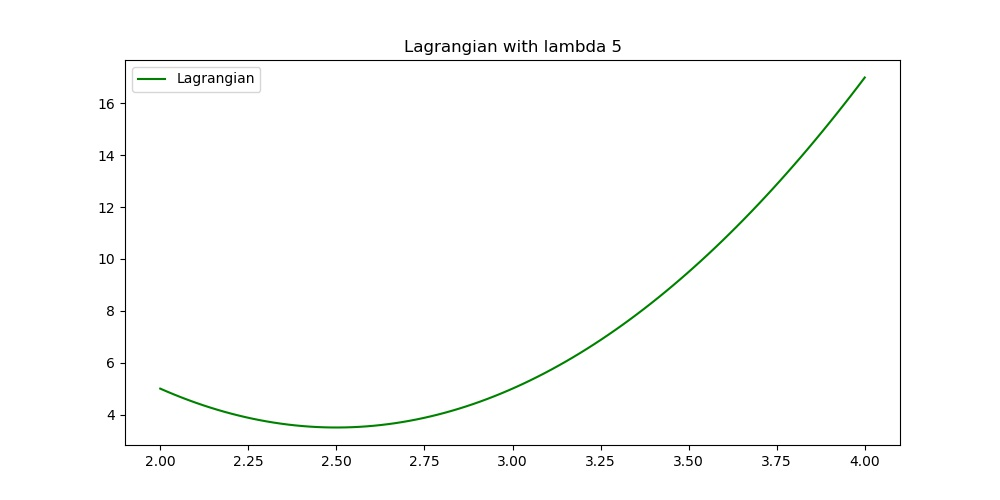
\includegraphics[width=10cm, height=5cm]{7c-lam5.jpg}
        \captionof{figure}{Plot of Lagrangian with $\lambda=5$} 
        }
        {\centering
        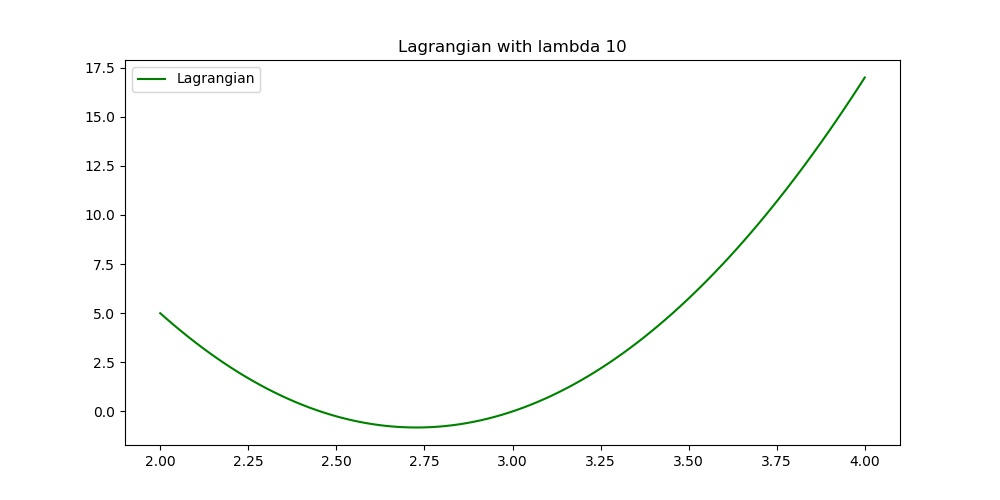
\includegraphics[width=10cm, height=5cm]{7c-lam10.jpg}
        \captionof{figure}{Plot of Lagrangian with $\lambda=10$} 
        }

        \subsection{(d)}
        {\centering
        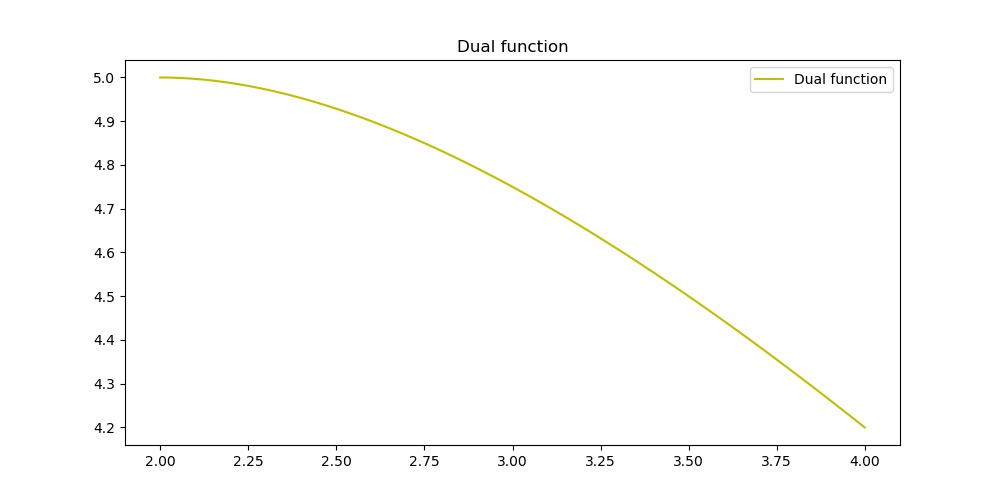
\includegraphics[width=10cm, height=5cm]{7d.jpg}
        \captionof{figure}{Plot of Dual function} 
        }

        \subsection{(e)}
        The dual problem is
        $$
        \mathop{\text{maximize}}_{\lambda} \frac{-\lambda^{3} +
        8\lambda^{2} + 10\lambda + 1}{(\lambda+1)^{2}}, \quad
        \text{subject to } \lambda \geq 0
        $$
        \indent And the maximizer $\lambda^{\star} = 2$, accordingly
        $d(\lambda^{\star}) = 5$.\\
        \indent Strong duality holds because the value of primal problem
        $p^{\star}$ is \textbf{5} and the value of dual problem $d^{\star}$
        is \textbf{5}.
    \end{framed}

    %%%%%%%%%%%%%%%%%%%%%%%%%%%%%%%%%%%%%%   Q8   %%%%%%%%%%%%%%%%%%%%%%%%%%%%%%%%%%%%%%%%%
    \begin{framed}
        \section{[Q8]}
        From (2), it is an unconstrained problem, take the derivative of $x$,
        we can have,
        \begin{align}
            \nabla f(\boldsymbol{x}) + 2\alpha \boldsymbol{A}^{T}
            (\boldsymbol{A}\boldsymbol{x}-b) &= 0\\
            \nabla f(\tilde{\boldsymbol{x}}) + 2\alpha \boldsymbol{A}^{T}
            (\boldsymbol{A}\tilde{\boldsymbol{x}}-b) &= 0\\
            \nabla f(\tilde{\boldsymbol{x}}) + \boldsymbol{A}\tilde{\boldsymbol{\upsilon}} &= 0
        \end{align}
        \indent where $\tilde{\boldsymbol{x}}$ is the solution to (2), and $\tilde{\boldsymbol{\upsilon}}=
        2\alpha(\boldsymbol{A} \tilde{\boldsymbol{x}} - \boldsymbol{b})$.

        From (1), it is a contrained problem, the Lagrangian is,
        \begin{align}
            L(\boldsymbol{x}, \boldsymbol{\upsilon}) &= f(\boldsymbol{x}) + 
            \boldsymbol{\upsilon} (\boldsymbol{A} \boldsymbol{x} - \boldsymbol{b})
        \end{align}
        \indent Take derivative with respect to $\boldsymbol{x}$, we have,
        \begin{equation}
            \nabla f(\boldsymbol{x}) + \boldsymbol{A} \boldsymbol{\upsilon} = 0
        \end{equation}
        \indent Note that a possible solution to (78) is exactly solution to
        (76) which is $\tilde{\boldsymbol{x}}, \tilde{\boldsymbol{\upsilon}}$,
        and again assume the optimal value to make
        dual problem maximum is ${\boldsymbol{\upsilon}}^{\star}$,  and 
        $\boldsymbol{x}^{\star}$ is exact the value to make
        primal problem maximum, hence we can have,
        \begin{align}
            d(\tilde{\boldsymbol{\upsilon}}) &\leq 
            d(\boldsymbol{\upsilon}^{\star}) \\
            &\leq f(\boldsymbol{x}^{\star})
        \end{align}
        \indent Hence, the lower bound of primal problem is
        \begin{align}
            d(\boldsymbol{\tilde{\upsilon}}) &\leq f(\boldsymbol{x}^{\star})
        \end{align}
    \end{framed}

     %%%%%%%%%%%%%%%%%%%%%%%%%%%%%%%%%%%%%%   Q9   %%%%%%%%%%%%%%%%%%%%%%%%%%%%%%%%%%%%%%%%%
    \begin{framed}
        \section{[Q9]}
        \subsection{(a)}
        $$
        \mathcal{L}(\boldsymbol{x}, \boldsymbol{\lambda}, \upsilon) = \left[ 
            -\sum\limits_{n=1}^{N} \log_{2}(\alpha_{n}+x_{n}) - \boldsymbol{\lambda}
            \boldsymbol{x} + \upsilon(\mathbf{1}^{T} \boldsymbol{x}-1)
        \right]
        $$
        \indent The KKT conditions are as follows,
        \begin{align}
            -x_{n} &\leq 0, n=1,\cdots, N\\
            \mathbf{1}^{T}\boldsymbol{x} - 1 &= 0\\
            \lambda_{n} &\geq 0, n=1,\cdots, N\\
            -\lambda_{n}x_{n} &= 0, n=1, \cdots, N\\
            -\frac{1}{\ln(2)(\alpha_{n} + x_{n})} - \lambda_{n} + \upsilon &= 0, n=1,
            \cdots, N
        \end{align}
        \indent From K3 and K4, we can get,
        \begin{align}
            x_{n}^{\star} = \frac{\lambda^{\star} \alpha_{n} + \frac{1}{\ln2}}
            {\upsilon^{\star}} - \alpha_{n}
        \end{align}

        \subsection{(b)}
        We could have,
        \begin{align}
            x_{n} \left( \upsilon  - \frac{1}{\ln(2) (\alpha_{n}
            +x_{n})} \right) &= 0\\
            \upsilon \geq \frac{1}{\ln(2) (\alpha_{n}+ x_{n})}
        \end{align}

        If $\upsilon < \frac{1}{\ln(2) (\alpha_{n} + x_{n})}$, to
        satisfy (77), $x_{n} >0$, hence,
        \begin{align}
            x_{n} = \frac{1}{\ln(2) \upsilon} - \alpha_{n}
        \end{align}

        If $\upsilon \geq \frac{1}{\ln(2) \alpha_{n}} > \frac{1}
        {\ln(2) (\alpha_{n}+ x_{n})}$,
        \begin{align}
            x_{n} = 0
        \end{align}

        \indent Hence,
            \begin{align}
                x^{\star}_{n} &= \max \left\{ 0, -\alpha_{n} + 
                \frac{1}{\ln(2) \upsilon^{\star}} \right\}\\
                \lambda^{\star}_{n} &= \max \left\{ 
                    0, \upsilon^{\star} - \frac{1}{\ln(2)\alpha_{n}}
                \right\}\\
                \sum\limits_{n} &\max \left\{ 0, -\alpha_{n} + 
                \frac{1}{\ln(2) \upsilon^{\star}} \right\} = 1
            \end{align}


        \subsection{(c)}
        Given $\upsilon^{\star}$, we can use,
        \begin{align}
            \sum\limits_{n} &\max \left\{ 0, -\alpha_{n} + 
            \frac{1}{\ln(2) \upsilon^{\star}} \right\} = 1
        \end{align}
        \indent Then we can get $x^{\star}_{n}$ and $\lambda_{n}^{\star}$ using equations
         from (b).

         \subsection{(d)}
         \begin{align}
            \sum\limits_{n} &\max \left\{ 0, -\alpha_{n} + 
            \frac{1}{\ln(2) \upsilon^{\star}} \right\} = 1
        \end{align}
        \indent Here is the algorithm to solve this problem,


        \begin{algorithm}[H]
            \SetAlgoLined
            \KwData{Set $\mathbf{D} = \left\{ \alpha_{i} \right\}_{i=1}^{N}$}
            \KwResult{$\upsilon^{\star}$}
            $\upsilon_{1} = \frac{N}{\ln(2) (1+\sum_{i=1}^{N} \alpha_{i})}$\;
            Sort $\mathbf{D}$ in ascending order\;
            i=1\;
            
            \While{$\upsilon_{i} \leq \frac{1}{\ln(2) \cdot \alpha_{i}}$}{

                $\alpha_{i}=0$\;
                $N=N-1$\;
                $i=i+1$\;
                $\upsilon_{i}=\frac{N}{\ln(2)(1+\sum_{i} \alpha_{i}) }$\;
            }
        \caption{Algorithm to find $\upsilon^{\star}$}
        \end{algorithm}
        \indent Note that in step 8, $\sum_{i} \alpha_{i}$ means you
        should add all elements in set $\mathbf{D}$ while $N=N-1$.
        \indent Briefly sepeaking, in the intial state, I assume all the 
        patch needs to be filled with water, and then iterates, in
        the iteration, I always remove the patch which has the highest
        ground level $\alpha_{i}$ until i can found the patch which satisfy
        $\sum\limits_{n} -\alpha_{n} + 
        \frac{1}{\ln(2) \upsilon^{\star}}=1$.

        \subsection{(e)}
        {\centering
        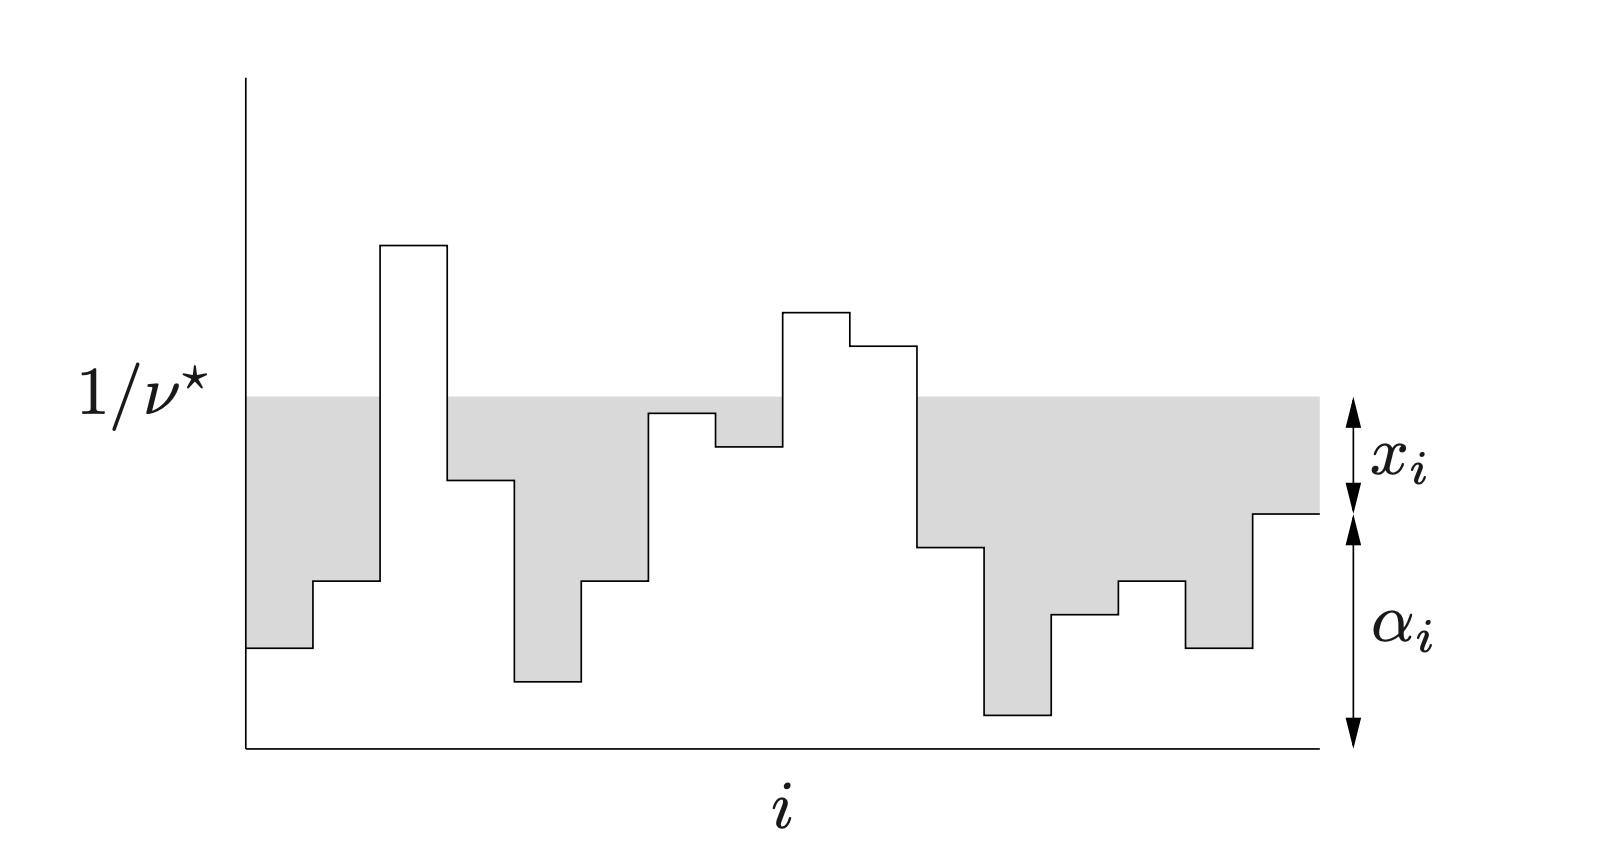
\includegraphics[width=10cm, height=5cm]{Q9_e.png}
        \captionof{figure}{Relation between $\alpha_{n},
        x^{\star}_{n} \text{ and } \upsilon^{\star}$} 
        }
        We think of $\alpha_{i}$ as the ground level 
        above patch $i$, and then flood the region with
        water to a depth of $\frac{1}{\upsilon}$, as illustrated
        in Figure(6), The total amount of water used is then
        $\sum_{i}^{n} \max \left\{ 0, -\alpha_{i} + 
        \frac{1}{\ln(2) \upsilon^{\star}} \right\}$. We then increase
        the flood level until we have used  a total amount of water
        equal to one. The depth of water above patch $i$ is then
        the optimal value $x^{\star}$
    \end{framed}

     %%%%%%%%%%%%%%%%%%%%%%%%%%%%%%%%%%%%%%   Q10   %%%%%%%%%%%%%%%%%%%%%%%%%%%%%%%%%%%%%%%%%
    \begin{framed}
        \section{[Q10]}
        \subsection{(a)}
        {\centering
        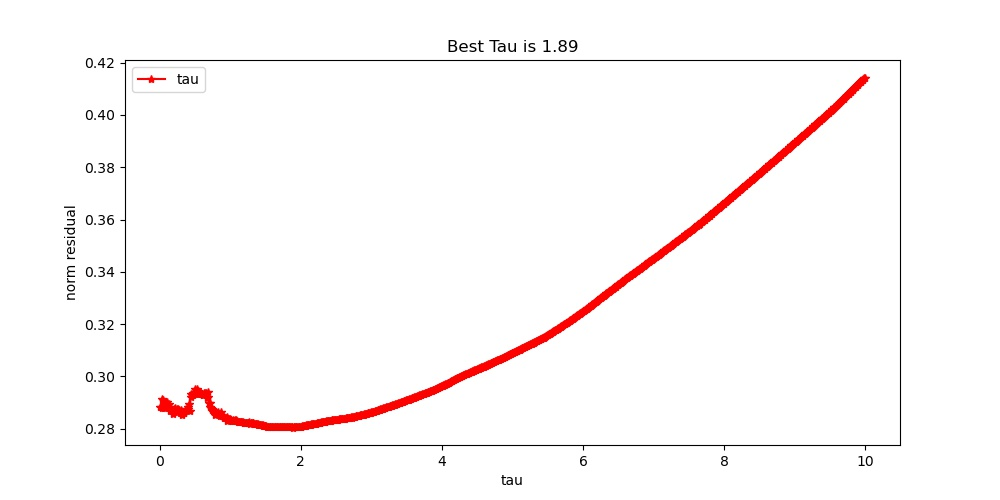
\includegraphics[width=10cm, height=5cm]{Q10_1.jpg}
        \captionof{figure}{Best $\tau$} 
        }
        \indent Here I set $\tau$ from 0.01 to 10, and calculate the norm residual.
        I found the best $\tau$ is \textbf{1.89} as is indicated in Figure(7).

        \subsection{(b)}
        {\centering
        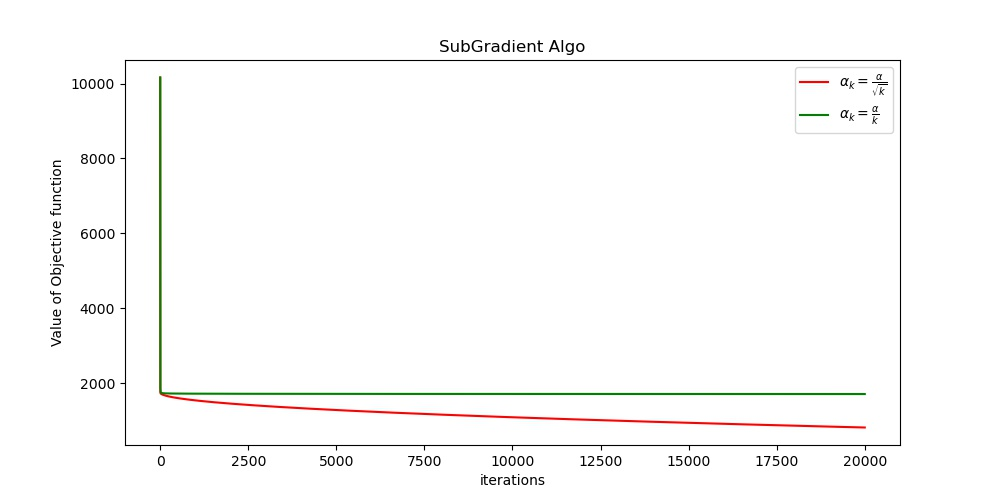
\includegraphics[width=10cm, height=5cm]{Q10_2.jpg}
        \captionof{figure}{Subgradient Descent} 
        }
        Here, If set $\alpha_{k}$ as fixed, it's not guaranteed that it can 
        converge. And If we set $\alpha_{k}=\frac{\alpha}{\sqrt{k}}$ and $\alpha_{k}
        =\frac{\alpha}{k}$, it converges as shown in Figure(8).

        \subsection{(c)}
        {\centering
        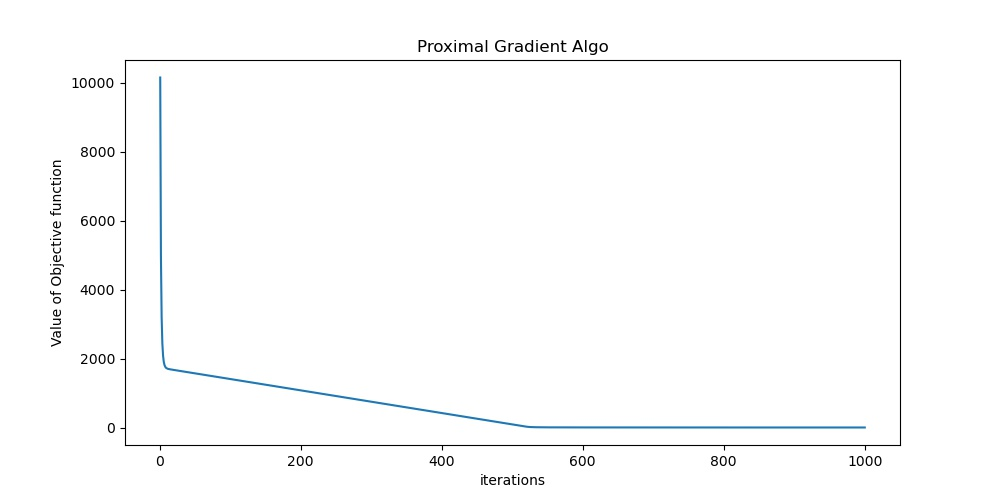
\includegraphics[width=10cm, height=5cm]{Q10_3.jpg}
        \captionof{figure}{Proximal Gradient Descent} 
        }

        \subsection{(d)}
        {\centering
        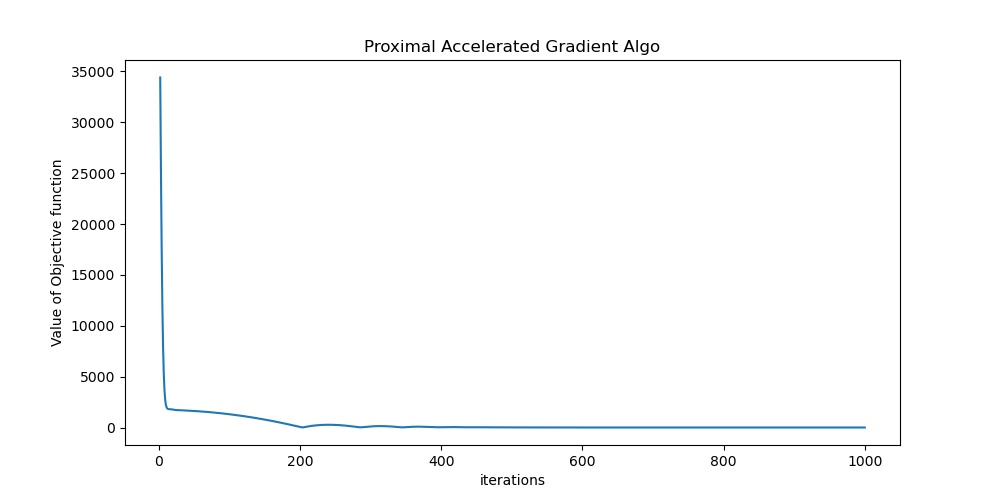
\includegraphics[width=10cm, height=5cm]{Q10_4.jpg}
        \captionof{figure}{Proximal Gradient Descent with acceleration} 
        }
    \end{framed}

    \begin{framed}
        \section{Appendix}
        All the source code can be found from
        \href{https://github.com/masqueraderx}{my personal Github}.
        \subsection{Q7}
        \begin{python}
import numpy as np
from matplotlib import pyplot as plt

def func(x):
    return x**2 + 1

def contraint(x):
    return (x-2) * (x-4)

def lagrange(x, lam):
    return func(x) + lam * contraint(x)

def dual(x):
    numerator = -x**3 + 8 * x**2 + 10 * x + 1
    denumerator = (x + 1)**2
    return numerator / denumerator

def plotObj(x, y):
    plt.figure(figsize=(10, 5))
    plt.plot(x, np.zeros(len(x)), 'bo', label='feasible set')
    plt.plot(x, y, 'r', label='objective function')
    plt.title('objective function')
    plt.xlim([1.0, 5.0])
    plt.ylim([-0.01, 20])
    plt.legend()
    plt.savefig('./hw05/7c.jpg')

def plotLagrange(x, y, lam):
    plt.figure(figsize=(10, 5))
    plt.plot(x, y, 'g', label='Lagrangian')
    plt.title('Lagrangian with lambda {}'.format(lam))
    plt.legend()
    plt.savefig('./hw05/7c-lam{}.jpg'.format(lam))

def plotDual(x, y):
    plt.figure(figsize=(10, 5))
    plt.plot(x, y, 'y', label='Dual function')
    plt.title('Dual function')
    plt.legend()
    plt.savefig('./hw05/7d.jpg')


if __name__ == '__main__':
    x = np.linspace(2,4,100)
    y = func(x)
    plotObj(x, y)
    for lam in [0, 5, 10]:
        L = lagrange(x, lam)
        plotLagrange(x, L, lam)
    d = dual(x)
    plotDual(x, d)
        \end{python}

        \subsection{Q10}
        \begin{python}
import numpy as np
import cvxpy as cp
import random
import os
from matplotlib import pyplot as plt

def Q10_a():
    res = []
    for tau in np.arange(0.01, 10, 0.01):
        x = cp.Variable(N)
        cost = 0.5 * cp.sum_squares(y - A @ x) + tau * cp.norm(x, 1)
        prob = cp.Problem(cp.Minimize(cost))
        prob.solve()
        res.append(cp.norm(x.value - x0, p=2).value)
    optimal_tau = (res.index(min(res)) + 1) /100
    return res, optimal_tau

def funcValue(tau, A, x, y):
    var = y - A @ x
    return 0.5 * np.linalg.norm(x=var, ord=2) ** 2 + tau * np.linalg.norm(x=x, ord=1)

def subGradient(alpha, tau, A, x, y, maxiter, delta, flag):
    k = 1
    x = np.mat(x).T #(N ,1)
    y = np.mat(y).T #(M, 1)
    A = np.mat(A) #(M, N)
    value = []
    iteration = []
    while (k < maxiter) and (np.linalg.norm(x - np.mat(x0)) > delta):
        dk = A.T @ (A @ x - y) + tau * np.sign(x) #(N, 1)
        if flag:
            x = x - alpha * dk / np.sqrt(k) # (N, 1)
        else:
            x = x - alpha * dk / k
        value.append(funcValue(tau, A, x, y))
        iteration.append(k)
        k += 1
        print(x.flatten())
    return x, value, iteration

def Proximal(alpha, tau, A, x, y, maxiter, delta):
    def T(x):
        for i in range(len(x)):
            if x[i] >= tau * alpha:
                x[i] = x[i] - tau * alpha
            elif abs(x[i]) <= tau * alpha:
                x[i] = 0
            elif x[i] <= - tau * alpha:
                x[i] = x[i] + tau * alpha
            else:
                return -1
        return x
    k = 0
    x = np.mat(x).T #(N ,1)
    y = np.mat(y).T #(M, 1)
    A = np.mat(A) #(M, N)
    fValue = []
    iteration = []
    while (k < maxiter) and (np.linalg.norm(x - np.mat(x0)) > delta):
        x = T(x + alpha * A.T @ (y - A @ x))
        k += 1
        print(x.flatten())
        fValue.append(funcValue(tau, A, x, y))
        iteration.append(k)
    return x, fValue, iteration


def accrProximal(alpha, tau, A, x, y, maxiter, delta):
    def Tec(x):
        for i in range(len(x)):
            if x[i] >= tau * alpha:
                x[i] = x[i] - tau * alpha
            elif abs(x[i]) <= tau * alpha:
                x[i] = 0
            elif x[i] <= - tau * alpha:
                x[i] = x[i] + tau * alpha
            else:
                return -1
        return x
    k = 1
    pk = np.mat(np.zeros(N)).T #(N, 1)

    x = [np.mat(x).T] #(N ,1)
    y = np.mat(y).T #(M, 1)
    A = np.mat(A) #(M, N)

    gd = A.T @ (A @ (x[-1] + pk) - y) #(N, 1)
    fValue = []
    iteration = []
    while (k < maxiter) and (np.linalg.norm(x[-1] - np.mat(x0)) > delta):
        x.append(Tec(x[-1] + pk - alpha * gd))
        k += 1
        pk = ((k - 1) / (k + 2)) * (x[-1] - x[-2])
        gd = A.T @ (A @ (x[-1] + pk) - y)

        print(x[-1].flatten())
        fValue.append(funcValue(tau, A, x[-1], y))
        iteration.append(k)
    return x[-1], fValue, iteration

if __name__ == '__main__':
    np.random.seed(2021) # Set random seed so results are repeatable # Set parameters
    M = 100
    N = 1000
    S = 10
    # Define A and y
    A = np.random.randn(M, N) # (M, N)
    ind0 = np.random.choice(N, S, 0)
    x0 = np.zeros(N)
    x0[ind0] = np.random.rand(S) # (N, )
    y = A@x0 + .25*np.random.randn(M) # (M, )
    savepath = 'C:/gexueren/Desktop/hw05/hw05/hw05'
    
    ######################## Q1 #######################
    res, optimal_tau = Q10_a()
    plt.figure(figsize=(10,5))
    plt.plot(np.arange(0.01,10, 0.01), res, 'r-*', label='tau')
    plt.title('Best Tau is {}'.format(optimal_tau))
    plt.xlabel('tau')
    plt.ylabel('norm residual')
    plt.legend()
    plt.savefig(os.path.join(savepath, 'Q10_1.jpg'))

    ######################## Q2 #######################
    x = np.ones(N) # initial value (N, )
    _, fValue_0, iteration_0 = subGradient(alpha=0.001, tau=optimal_tau, A=A, x=x, y=y, maxiter=20000, delta=1e-3, flag=True)
    plt.figure(figsize=(10, 5))
    plt.plot(iteration_0, fValue_0, color='r', label=r'$\alpha_{k}= \frac{\alpha}{\sqrt{k}}$')

    x = np.ones(N) # initial value (N, )
    _, fValue_1, iteration_1 = subGradient(alpha=0.001, tau=optimal_tau, A=A, x=x, y=y, maxiter=20000, delta=1e-3, flag=False)
    plt.plot(iteration_1, fValue_1, color='g', label=r'$\alpha_{k}= \frac{\alpha}{k}$')
    plt.title('SubGradient Algo')
    plt.xlabel('iterations')
    plt.ylabel('Value of Objective function')
    plt.legend()
    plt.savefig(os.path.join(savepath, 'Q10_2.jpg'))

    ######################## Q3 #######################
    x = np.ones(N) # initial value (N, )
    _, fValue, iteration = Proximal(alpha=0.001, tau=optimal_tau, A=A, x=x, y=y, maxiter=1000, delta=1e-3)
    plt.figure(figsize=(10, 5))
    plt.plot(iteration, fValue)
    plt.title('Proximal Gradient Algo')
    plt.xlabel('iterations')
    plt.ylabel('Value of Objective function')
    plt.savefig(os.path.join(savepath, 'Q10_3.jpg'))

    ######################## Q4 #######################
    x = np.ones(N) # initial value (N, )
    _, fValue, iteration = accrProximal(alpha=0.0001, tau=optimal_tau, A=A, x=x, y=y, maxiter=1000, delta=1e-3)
    plt.figure(figsize=(10, 5))
    plt.plot(iteration, fValue)
    plt.title('Proximal Accelerated Gradient Algo')
    plt.xlabel('iterations')
    plt.ylabel('Value of Objective function')
    plt.savefig(os.path.join(savepath, 'Q10_4.jpg'))
        \end{python}
    \end{framed}
\end{document}